\section{Hardware}
The hardware used for this experiment are specially designed clusters made with Raspberry Pi's 3 model B+. These Pi's are assigned using the same ratio of FLPs and EPNs at CERN (1:6) and 1 Information Node. The Pi's are modified with an extra Ethernet port. The exact specifications are in table 5.1:

\begin{table}[htb]
\begin{tabular}{| l | l |}
\hline
Processor & Cortex-A53 1.4GHZ\\ \hline
RAM & 1GB LPDDR2 SDRAM\\ \hline
Network & 1 300MbE 1 10/100MbE \\ \hline
Operating System & Raspbian Stretch (Debian 9)\\ \hline
\end{tabular} 
\caption{Specifications modified Raspberry Pi 3 model B+}
\end{table}

Everything is setup and build from a single server unit. The IP addresses are also managed from this unit. Specifications are in table 5.2:

\begin{table}[htb]
\begin{tabular}{| l | l |}
\hline
Processor & Intel Xeon\\ \hline
RAM & \\ \hline
Network & \\ \hline
Operating System & Raspbian Stretch (Debian 9)\\ \hline
\end{tabular}
\caption{Specifications management server}
\end{table}

\newpage

The network configuration consists of a bidirectional connection of :
\begin{figure}[htb]
    \centering
    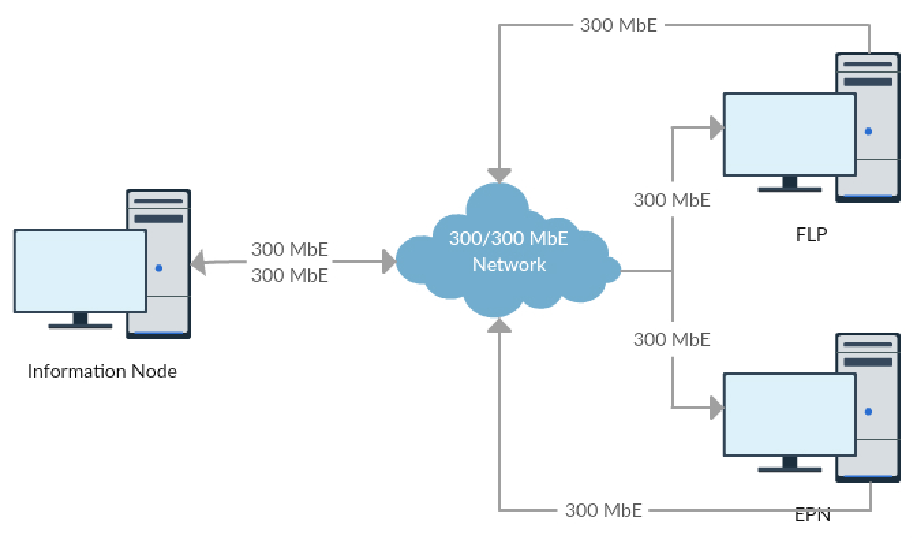
\includegraphics[scale=0.5]{./graphics/chapter5/Network_thesis.pdf}
    \caption{Network setup}
\end{figure}

\newpage

The clusters of pi's are build using a 

\section{Software}
The software used is found at https://github.com/SoftwareForScience/O2-Balancer. It consists of 3 executable programs to represent an FLP, EPN and Information Node. These programs are send to the devices to represent their respective units. Apart from that it uses a slightly modified version of FairRoot. Since only the FairMQ part is needed for the programs to run it has been split off from this code. The full FairRoot code can be found at \\ 
https://github.com/FairRootGroup/FairRoot and the split off part with only FairMQ can be found at
% FairMQ code invoegen wanneer officieel af gesplitst
. \\ 
The Infomation Node serves 2 purposes. At firs it generates the TFs that are send to the FLPs using FairMQ. It also receives notifications from the EPNs when they have received the full TF from the FLPs again. The configuration is done using YAML files. A diagram of the connections and dependencies are as followed.

%\begin{figure}[htb]
%    \centering
%    \textbf{Your title}\par\medskip
%    \includegraphics[scale=0.3]{}
%    \caption{Block diagram of the cluster connections (van der Heijden, 2018, p. 22)}
%\end{figure}

\begin{table}[htb]
\begin{tabular}{| l | l |}
\hline
Library/Tool & Version \\ \hline
FairMQ & \\ \hline
ZeroMQ & 4.2.5\\ \hline
Zookeeper & 3.4.9 \\ \hline
Cmake & 3.11.0 \\ \hline
Boost & 1.66.0 \\ \hline
Yaml-cpp & 0.5.2 \\ \hline
Compiler & gcc 6.3.0 20170516 (Raspbian 6.3.0-18+rpi1+deb9u1)\\ \hline
\end{tabular}
\caption{Dependencies software}
\end{table}

\section{Data analysis tools}
In order to stay consistent with the previous experiment, the same tools will be used to create and visualize the data. This can be found at \\ https://github.com/valvy/BalancerScripts. These scripts are written in Python and ROOT to generate graphs and histograms from the log files received from the software. The dependencies are specified in table 5.4.

\begin{table}[ht]
\begin{tabular}{| l | l |}
\hline
Tool & Version \\ \hline
Raspbian & Centos 7 \\ \hline
ROOT & 6.13.02 \\ \hline
Python & 2.7.13 \\ \hline
Ansible & 2.2.1 \\ \hline
\end{tabular}
\caption{Dependencies for the analysis scripts}
\end{table}

\newpage

\section{Experiments}
In order to check whether or not the Information Node has any issues with increased numbers of FLPs and EPNs, the same experiments need to be done use described in the previous report (van der Heijden, 2018, p23-p27) but will be briefly summarized again. The experiments are done in two steps. First the experiments need to be run using the same amount of FLPs and EPNs to verify whether or not the new setup of Pi clusters are able to give the same result. Second the experiments need to be run again using more FLPs and EPNs to check if it indeed does have an effect on the Information Node.

\subsection{Experiment one}
\textbf{Ticktime influence on the blacklist algorithm with one fail-over}
\\\\
The first experiment uses a fixed sample size to be send from the Information Node, and will have 1 fail-over during its run. This sample size is set to hundred-forty kilobyte and 
the heartbeat rate is set to twenty milliseconds. This heartbeat is set at the same rate used at CERN. This sample size is set to accommodate the slower Ethernet and processing speed of Raspberry Pi as compared to units used in the previous experiment (van der Heijden, 2018, p.23). \\
This experiment will disable one EPN when it recieves the first STF from hearbeat 3.000. Then special scripts will parse the logfiles between heartbeat 2.000 and 10.000 to have enough of a buffer to read from. A flowchart can be found in figure 4.3.

%\begin{figure}[htb]
%    \centering
%    \textbf{Your title}\par\medskip
%    \includegraphics[scale=0.3]{}
%    \caption{Flow char experiment (van der Heijden, 2018, p. 24)}
%\end{figure}

\subsection{Experiment two}
\textbf{Ticktime influence on the blacklist algorithm with all but one fail-over}
\\\\
The same heartbeat rate and sample size are used from experiment one. For this experiment the first EPN will disabled at heartbeat 2.000. After that every 1.000 heartbeats an additional EPN will be disabled until there is only 1 left. Scripts will parse all the logs to check how many TFs were lost during this progress. A flowchart can be found in figure 5.4.

%\begin{figure}[htb]
%    \centering
%    \textbf{Your title}\par\medskip
%    \includegraphics[scale=0.3]{}
%    \caption{Flow chart random init experiment (van der Heijden, 2018, p. 25)}
%\end{figure}

\subsection{Experiment three}
\textbf{Ticktime influence on the blacklist algorithm with all but one-fail over with random sample size}
\\\\
The same heartbeat rate is used from experiment one. A random sample size will be generated from the FLPs between .. \& .. . Apart from that the same configuration will be used as in experiment two. The first EPN will be disabled at heartbeat 2.000 and after that every 1.000 heartbeats an additional EPN will be disabled. A flowchart can be found in figure 5.5.

%\begin{figure}[htb]
%    \centering
%    \textbf{Your title}\par\medskip
%    \includegraphics[scale=0.3]{}
%    \caption{Flow chart random experiment (van der Heijden, 2018, p. 26)}
%\end{figure}